\documentclass[aspectratio=169, 11pt]{beamer}

% ── Tema y colores ────────────────────────────────────────────────────────────
\usetheme{Madrid}
\usecolortheme{default}
\definecolor{azuloscuro}{RGB}{31, 56, 100}
\definecolor{azulmedio}{RGB}{46, 117, 182}
\definecolor{verdeok}{RGB}{39, 80, 10}
\definecolor{rojoko}{RGB}{180, 57, 14}
\setbeamercolor{structure}{fg=azuloscuro}
\setbeamercolor{frametitle}{bg=azuloscuro, fg=white}
\setbeamercolor{title}{bg=azuloscuro, fg=white}
\setbeamercolor{block title}{bg=azulmedio, fg=white}
\setbeamercolor{block body}{bg=azuloscuro!5}
\setbeamercolor{item}{fg=azulmedio}
\setbeamertemplate{navigation symbols}{}
\setbeamertemplate{footline}{%
  \leavevmode\hbox{%
    \begin{beamercolorbox}[wd=.33\paperwidth,ht=2.5ex,dp=1ex,left]{author in head/foot}%
      \hspace*{2ex}\insertshortauthor
    \end{beamercolorbox}%
    \begin{beamercolorbox}[wd=.34\paperwidth,ht=2.5ex,dp=1ex,center]{title in head/foot}%
      \insertshorttitle
    \end{beamercolorbox}%
    \begin{beamercolorbox}[wd=.33\paperwidth,ht=2.5ex,dp=1ex,right]{date in head/foot}%
      \insertframenumber{}/\inserttotalframenumber\hspace*{2ex}
    \end{beamercolorbox}%
  }%
}

% ── Paquetes ──────────────────────────────────────────────────────────────────
\usepackage[utf8]{inputenc}
\usepackage[T1]{fontenc}
\usepackage[spanish]{babel}
\usepackage{booktabs}
\usepackage{graphicx}
\usepackage{amsmath}
\usepackage{colortbl}
\usepackage{tabularx}
\usepackage{tikz}

% ── Metadatos ─────────────────────────────────────────────────────────────────
\title[RD -- Pipeline Completo]{Clasificación Automática de\\Retinopatía Diabética}
\subtitle{Pipeline Completo de Gradación de Severidad}
\author[García, Véliz, Solano]{%
  Javier García Fernández \and
  Miguel Ángel Véliz Ayala \and
  Martín Solano Martínez}
\institute{Procesamiento de Imagen en Medicina --- Curso 2025/2026}
\date{24 de abril de 2026}

\begin{document}

% ══════════════════════════════════════════════════════════════════════════════
%  PORTADA
% ══════════════════════════════════════════════════════════════════════════════
\begin{frame}[plain]
  \titlepage
\end{frame}


% ══════════════════════════════════════════════════════════════════════════════
%  SECCIÓN 1: JAVIER — Problema, dataset, pipeline, baseline (~3.5 min)
% ══════════════════════════════════════════════════════════════════════════════
\section{Problema y Pipeline}

% ── Slide 1: Contexto clínico ────────────────────────────────────────────────
\begin{frame}{¿Qué es la retinopatía diabética?}
  % GUION JAVIER: "La retinopatía diabética es una complicación de la diabetes
  % que afecta a los vasos de la retina. Es una de las principales causas de
  % ceguera prevenible. El cribado manual de miles de retinografías es inviable,
  % por eso necesitamos un sistema automático."

  \begin{columns}[T]
    \begin{column}{0.52\textwidth}
      \begin{itemize}
        \item Complicación microvascular de la diabetes
        \item Principal causa de \textbf{ceguera prevenible}
        \item 540M de diabéticos, 35\,\% con afectación retiniana
        \item Cribado manual inviable $\to$ \textbf{gradación automática}
      \end{itemize}
    \end{column}
    \begin{column}{0.44\textwidth}
      \small
      \begin{tabular}{cl}
        \toprule
        \textbf{Grado} & \textbf{Lesiones clave} \\
        \midrule
        G0 & Sin lesiones \\
        G1 & Microaneurismas \\
        G2 & Hemorragias, exudados \\
        G3 & Anomalías venosas extensas \\
        G4 & Neovascularización \\
        \bottomrule
      \end{tabular}
    \end{column}
  \end{columns}
  \vspace{6pt}
  \centering
  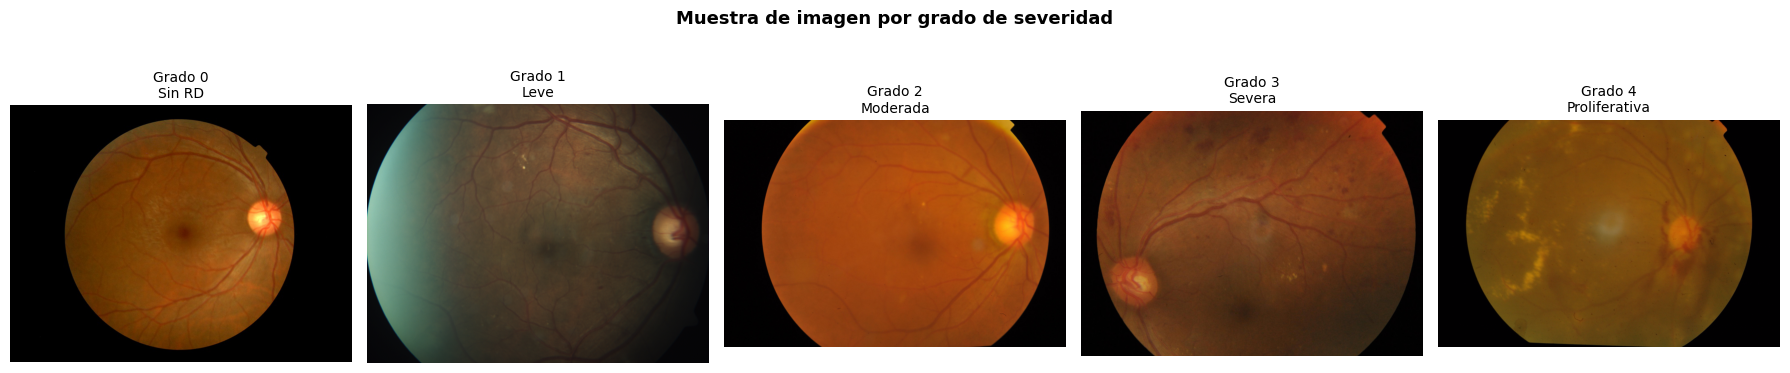
\includegraphics[width=0.82\textwidth]{figura1.png}
\end{frame}

% ── Slide 2: Dataset ─────────────────────────────────────────────────────────
\begin{frame}{Dataset: APTOS 2019}
  % GUION JAVIER: "Usamos APTOS 2019, 3662 retinografías de clínicas rurales
  % de la India. El principal problema es el desbalance: G0 es casi la mitad,
  % G3 solo el 5%. También usamos APTOS 2015 como fuente de datos adicional
  % para el preentrenamiento."

  \begin{columns}[T]
    \begin{column}{0.45\textwidth}
      \textbf{APTOS 2019} --- 3\,662 retinografías
      \vspace{4pt}

      \small
      \begin{tabular}{lrr}
        \toprule
        \textbf{Clase} & \textbf{Train} & \textbf{\%} \\
        \midrule
        G0 Sin RD       & 1\,434 & 48,9\,\% \\
        G1 Leve         & 300    & 10,2\,\% \\
        G2 Moderada     & 808    & 27,6\,\% \\
        \rowcolor{rojoko!15}
        G3 Severa       & 154    & \textbf{5,3\,\%} \\
        G4 Proliferativa & 234   & 8,0\,\% \\
        \bottomrule
      \end{tabular}
    \end{column}
    \begin{column}{0.52\textwidth}
      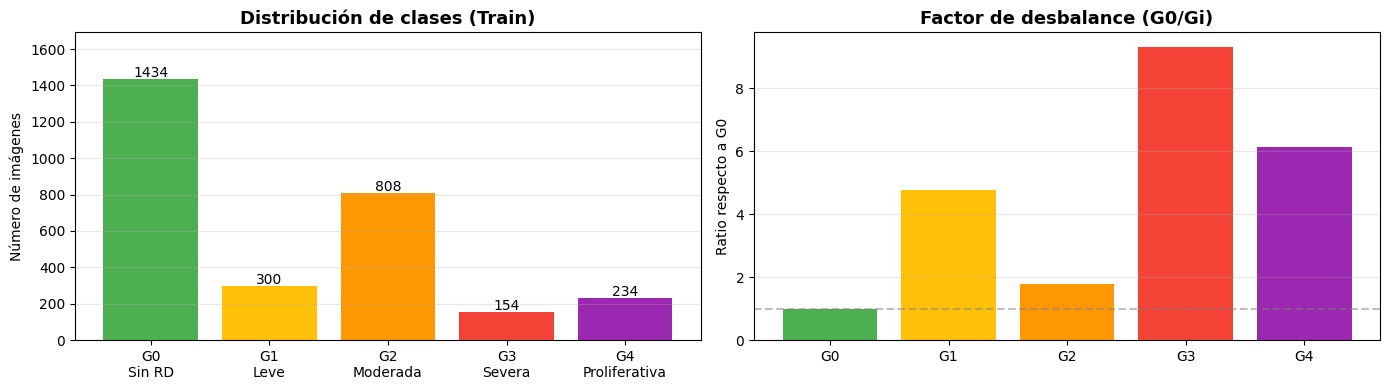
\includegraphics[width=\textwidth]{desbalance.png}
    \end{column}
  \end{columns}
\end{frame}

% ── Slide 3: Preprocesamiento y augmentación ─────────────────────────────────
\begin{frame}{Preprocesamiento y Data Augmentation}
  % GUION JAVIER: "El preprocesamiento tiene 4 pasos: máscara circular para
  % quitar el fondo negro, CLAHE para mejorar el contraste local, resize
  % y normalización ImageNet. En augmentación solo aplicamos transformaciones
  % que tienen sentido anatómico: flip horizontal sí, vertical NO porque
  % produce una retina imposible."

  \begin{columns}[T]
    \begin{column}{0.48\textwidth}
      \textbf{Preprocesamiento (4 pasos):}
      \begin{enumerate}
        \item \textbf{Máscara circular} --- canal verde
        \item \textbf{CLAHE} --- contraste local (LAB)
        \item \textbf{Resize} --- 224 o 384\,px
        \item \textbf{Normalización ImageNet}
      \end{enumerate}
      \vspace{4pt}
      {\small\textit{Nota:} Exp.~G sustituye CLAHE por Ben Graham.}
    \end{column}
    \begin{column}{0.48\textwidth}
      \textbf{Augmentación conservadora:}
      \begin{itemize}
        \item[\textcolor{verdeok}{\checkmark}] Flip horizontal, rotación $\pm 20^\circ$
        \item[\textcolor{verdeok}{\checkmark}] Zoom, ruido gaussiano, contraste
        \item[\textcolor{rojoko}{$\times$}] Flip vertical (anatomía imposible)
        \item[\textcolor{rojoko}{$\times$}] Rotación $>30^\circ$
        \item[\textcolor{rojoko}{$\times$}] Padding zeros (crea shortcuts)
      \end{itemize}
    \end{column}
  \end{columns}
\end{frame}

% ── Slide 4: Métricas y Baseline ─────────────────────────────────────────────
\begin{frame}{Baseline y métricas}
  % GUION JAVIER: "Usamos kappa cuadrático ponderado como métrica principal
  % porque penaliza más confundir G0 con G4 que con G1, y F1 macro para
  % detectar fallos en clases minoritarias. El baseline es EfficientNet-B3
  % a 224px con CrossEntropy ponderada. Consigue un kappa de 0.862 que es
  % bueno, pero al mirar la matriz de confusión vemos que las confusiones
  % están entre grados adyacentes: ordena bien la gravedad pero no acierta
  % la etiqueta exacta."

  \begin{columns}[T]
    \begin{column}{0.45\textwidth}
      \textbf{Métricas:}
      \begin{itemize}
        \item $\kappa^2$: penaliza $(i{-}j)^2$ $\to$ alineada con gravedad clínica
        \item F1 macro: detecta fallos en minoritarias
      \end{itemize}
      \vspace{6pt}
      \textbf{Baseline:}
      \begin{itemize}
        \item EfficientNet-B3 (MONAI, ImageNet)
        \item 224$\times$224\,px, 20 épocas
        \item Weighted CrossEntropy
      \end{itemize}
      \vspace{6pt}
      \begin{block}{Resultados baseline}
        $\kappa^2 = 0{,}862$ \quad F1 $= 0{,}602$
      \end{block}
    \end{column}
    \begin{column}{0.52\textwidth}
      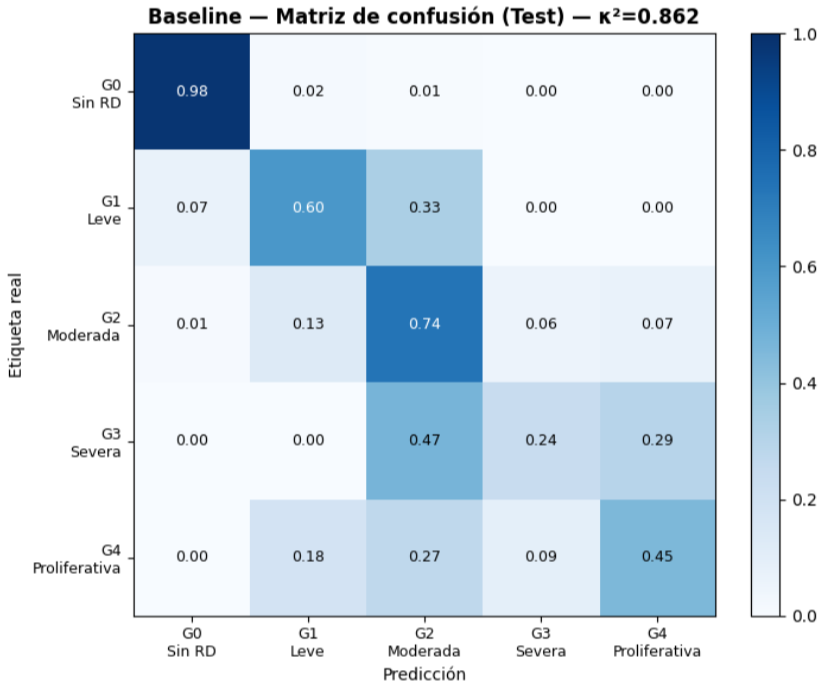
\includegraphics[width=\textwidth]{baseline_conf_matrix.png}
    \end{column}
  \end{columns}
\end{frame}

% ── Slide 5: Limitaciones del baseline ───────────────────────────────────────
\begin{frame}{Limitaciones identificadas}
  % GUION JAVIER: "Del análisis del baseline sacamos tres limitaciones claras
  % que motivan los experimentos posteriores. Y paso el turno a Miguel que
  % va a explicar cómo las atacamos."

  \begin{enumerate}
    \item[\textbf{L1.}] \textbf{Desbalance de clases} --- G3 solo tiene 154
          imágenes, la CrossEntropy ponderada no es suficiente.
          $\to$ \textit{Exp.~A, D, E, J}
    \item[\textbf{L2.}] \textbf{Resolución insuficiente} --- un microaneurisma
          a 224\,px $=$ 1--3 píxeles, al borde de desaparecer.
          $\to$ \textit{Exp.~F}
    \item[\textbf{L3.}] \textbf{Pérdida desalineada} --- CrossEntropy trata
          las clases como independientes, pero $\kappa^2$ penaliza la
          distancia ordinal. El gradiente no empuja hacia lo que se mide.
          $\to$ \textit{Exp.~F}
  \end{enumerate}

  \vspace{8pt}
  \centering
  \textit{Además, las debilidades se descubren iterativamente:}\\
  \textit{el Grad-CAM de F motiva G, los resultados de B motivan I\ldots}
\end{frame}

% ══════════════════════════════════════════════════════════════════════════════
%  SECCIÓN 2: MIGUEL — Exp. A, D, E, F (~3.5 min)
% ══════════════════════════════════════════════════════════════════════════════
\section{Experimentos: Desbalance y Regresión Ordinal}

% ── Slide 6: Exp A ───────────────────────────────────────────────────────────
\begin{frame}{Exp.~A --- Sobremuestreo}
  % GUION MIGUEL: "Para atacar el desbalance, la primera idea es dar más
  % peso a las clases minoritarias replicando sus muestras. El kappa sube
  % a 0.88 y G2 es la gran beneficiaria. Pero G3 apenas mejora: replicar
  % 154 imágenes no añade información nueva. Lo que necesitamos es variedad,
  % no volumen. Esto lo resuelve el Exp J con datos externos."

  \begin{columns}[T]
    \begin{column}{0.55\textwidth}
      \textbf{Problema:} Desbalance de clases (L1).\\
      \textbf{Acción:} WeightedRandomSampler para batches equilibrados.

      \vspace{6pt}
      \begin{block}{Resultados}
        $\kappa^2 = 0{,}880$ \quad F1 $= 0{,}631$
      \end{block}

      \begin{itemize}
        \item G2 sube de F1=0,72 a \textbf{0,78}
        \item G3 apenas mejora (0,28 $\to$ 0,29)
        \item El modelo se atreve más, no se refugia en G0
      \end{itemize}
    \end{column}
    \begin{column}{0.4\textwidth}
      \begin{alertblock}{Lección}
        Replicar datos $\neq$ añadir información.\\[4pt]
        G3 necesita \textbf{variedad} (más centros, más equipos), no volumen.
      \end{alertblock}
    \end{column}
  \end{columns}
\end{frame}

% ── Slide 7: Exp D y E ──────────────────────────────────────────────────────
\begin{frame}{Exp.~D y E --- Pipelines jerárquicos}
  % GUION MIGUEL: "La segunda estrategia es dividir el problema. En vez de
  % un modelo que haga todo, usamos una estructura en árbol. El Exp D separa
  % primero sano de enfermo y luego gradúa. El resultado es el mejor F1 del
  % proyecto empatado con A, y sobre todo sube mucho G4 que es la clase más
  % peligrosa clínicamente. Esta estructura refleja cómo trabaja un
  % oftalmólogo: primero screening, luego grading."

  \begin{columns}[T]
    \begin{column}{0.5\textwidth}
      \textbf{Exp.~D --- Dos etapas:}
      \begin{enumerate}
        \item ¿Tiene RD? (G0 vs resto)
        \item ¿Qué grado? (G1--G4)
      \end{enumerate}

      \vspace{4pt}
      \textbf{Exp.~E --- Tres niveles:}
      \begin{enumerate}
        \item ¿Sano?
        \item ¿Mild o Severe?
        \item Grado final
      \end{enumerate}
    \end{column}
    \begin{column}{0.47\textwidth}
      \small
      \begin{tabular}{lcc}
        \toprule
        & $\kappa^2$ & F1 \\
        \midrule
        D & 0,860 & \textbf{0,631} \\
        E & 0,855 & 0,602 \\
        \bottomrule
      \end{tabular}

      \vspace{8pt}
      \begin{block}{G4 Proliferativa}
        F1: 0,51 (baseline) $\to$ \textbf{0,59} (Exp.~D)\\
        \textbf{+16\,\%} en la clase más crítica.
      \end{block}
    \end{column}
  \end{columns}
\end{frame}

% ── Slide 8: Exp F ───────────────────────────────────────────────────────────
\begin{frame}{Exp.~F --- 384\,px + Regresión ordinal}
  % GUION MIGUEL: "Aquí hacemos dos cambios importantes. Primero, subimos
  % la resolución a 384px para ver mejor los microaneurismas. Segundo,
  % dejamos de tratar los grados como clases independientes y los tratamos
  % como una progresión continua con MSELoss, que tiene la misma forma
  % que kappa cuadrático. Los umbrales se optimizan con Nelder-Mead.
  % El kappa es bueno, 0.872, pero hay un problema grave: de 33 casos
  % de G4 en test, solo detecta 3. La MSELoss con desbalance comprime
  % las predicciones hacia el centro."

  \begin{columns}[T]
    \begin{column}{0.5\textwidth}
      \textbf{Cambios respecto al baseline:}
      \begin{itemize}
        \item Resolución: 224 $\to$ \textbf{384\,px}
        \item Cabeza: 5 neuronas $\to$ \textbf{1 neurona} (continua)
        \item Pérdida: CrossEntropy $\to$ \textbf{MSELoss}
        \item Post-proceso: argmax $\to$ \textbf{umbrales Nelder-Mead}
      \end{itemize}

      \begin{block}{Resultados}
        $\kappa^2 = 0{,}872$ \quad F1 $= 0{,}507$
      \end{block}
    \end{column}
    \begin{column}{0.47\textwidth}
      \begin{alertblock}{Problema grave: G4}
        De 33 imágenes de G4 en test,\\
        \textbf{solo detecta 3} (recall = 9\,\%).\\[4pt]
        MSELoss + desbalance $\to$\\
        compresión hacia el centro.
      \end{alertblock}
      \vspace{4pt}
      {\small Al analizar Grad-CAM se observa un
       comportamiento mixto que motiva el Exp.~G.}
    \end{column}
  \end{columns}
\end{frame}

% ══════════════════════════════════════════════════════════════════════════════
%  SECCIÓN 3: MARTÍN — Exp. B, C, G, I, J + Conclusiones (~3 min)
% ══════════════════════════════════════════════════════════════════════════════
\section{Baselines alternativos, interpretabilidad y conclusiones}

% ── Slide 9: Exp B y C ──────────────────────────────────────────────────────
\begin{frame}{Exp.~B y C --- ¿Hace falta el deep learning?}
  % GUION MARTÍN: "Antes de seguir mejorando el CNN, nos preguntamos: ¿hace
  % falta? El Exp B usa radiómica clásica con 107 features y regresión
  % logística L1. El kappa es 0.72, modesto, pero lo valioso es la
  % interpretabilidad: podemos leer qué features importan para cada grado.
  % El Exp C usa BiomedCLIP sin entrenar nada: kappa 0.71 con prompts
  % simples. Ambos quedan 14-15 puntos por debajo del CNN. Conclusión:
  % sí necesitamos entrenar un modelo específico."

  \begin{columns}[T]
    \begin{column}{0.48\textwidth}
      \textbf{Exp.~B --- Radiómica + LR L1}
      \begin{itemize}
        \item 107 features (PyRadiomics)
        \item $\kappa^2 = 0{,}722$ \quad F1 $= 0{,}479$
        \item Valor: \textbf{interpretabilidad}
        \item Ej: \texttt{10Percentile} $\to$ hemorragias
      \end{itemize}
    \end{column}
    \begin{column}{0.48\textwidth}
      \textbf{Exp.~C --- BiomedCLIP zero-shot}
      \begin{itemize}
        \item Sin entrenamiento en APTOS
        \item Prompts simples: $\kappa^2 = 0{,}711$
        \item Prompts clínicos: $\kappa^2 = 0{,}515$
        \item Valor: confirma que \textbf{el ajuste fino es imprescindible}
      \end{itemize}
    \end{column}
  \end{columns}

  \vspace{8pt}
  \centering
  \begin{block}{}
    \centering
    Ambos quedan \textbf{14--15 puntos} por debajo del CNN $\to$ el deep learning sí aporta.
  \end{block}
\end{frame}

% ── Slide 10: Exp G ─────────────────────────────────────────────────────────
\begin{frame}{Exp.~G --- Ben Graham: mejor métrica, peor interpretabilidad}
  % GUION MARTÍN: "Al ver que el Grad-CAM de F tenía comportamiento mixto,
  % aplicamos el filtro de Ben Graham, que es un paso alto que quita la
  % iluminación de fondo. El kappa sube a 0.882, el mejor del proyecto
  % en ese momento. PERO al hacer Grad-CAM del modelo G, las activaciones
  % empeoran: se van a la periferia. ¿Por qué? Porque Grad-CAM visualiza
  % la última capa a 7x7 píxeles, y a esa resolución lo que domina son
  % los bordes de alto contraste que Graham amplifica. Este es el hallazgo
  % más importante: mejor métrica no significa modelo más fiable."

  \begin{columns}[T]
    \begin{column}{0.5\textwidth}
      \textbf{Acción:}
      \begin{itemize}
        \item Filtro Ben Graham (paso alto)
        \item Máscara dura a nivel de tensor
        \item Aug.\ solo fotométricas
      \end{itemize}

      \begin{block}{Resultados}
        $\kappa^2 = 0{,}882$ (+0,01 vs F)\\
        F1 $= 0{,}575$
      \end{block}

      \vspace{4pt}
      \begin{alertblock}{Hallazgo clave}
        Grad-CAM \textbf{empeora} respecto a F.\\
        $\kappa^2 \uparrow$ pero interpretabilidad $\downarrow$
      \end{alertblock}
    \end{column}
    \begin{column}{0.47\textwidth}
      
\includegraphics[width=\textwidth]{grad_cam_exp_F.png}
      {\tiny Grad-CAM Exp.~F: comportamiento mixto.}
    \end{column}
  \end{columns}
\end{frame}

% ── Slide 11: Exp I y J ─────────────────────────────────────────────────────
\begin{frame}{Exp.~I y J --- Fusión y preentrenamiento}
  % GUION MARTÍN: "El Exp I fusiona las 1536 deep features del CNN con las
  % 107 radiómicas. El 96.5% de la aportación es del CNN, pero la radiómica
  % ayuda en las clases difíciles: el F1 sube a 0.631. El Exp J es el que
  % da el mejor kappa del proyecto: 0.885. Preentrenamos 20 épocas en las
  % 35 mil imágenes de APTOS 2015 y fine-tuneamos en 2019. Lo revelador
  % es que desde la primera época de fine-tuning ya alcanza 0.883: el modelo
  % ya sabe qué es una retina, solo ajusta detalles. Es mucho más resiliente."

  \begin{columns}[T]
    \begin{column}{0.48\textwidth}
      \textbf{Exp.~I --- Fusión CNN + Radiómica}
      \begin{itemize}
        \item 1\,536 deep + 107 radiómicas
        \item $\kappa^2 = 0{,}855$ \quad F1 $= 0{,}631$
        \item 96,5\,\% del peso es CNN
        \item Radiómica ayuda en G1, G3
      \end{itemize}
    \end{column}
    \begin{column}{0.48\textwidth}
      \textbf{Exp.~J --- Pretrain APTOS 2015}
      \begin{itemize}
        \item 35\,k imgs $\to$ fine-tune 2019
        \item $\kappa^2 = \mathbf{0{,}885}$ \quad F1 $= 0{,}551$
        \item \textbf{Mejor $\kappa^2$ del proyecto}
        \item Época 1 de FT: ya $\kappa^2 = 0{,}883$
        \item Recall G4: 9\,\% $\to$ 27\,\%
      \end{itemize}
    \end{column}
  \end{columns}

  \vspace{6pt}
  \centering
  {\small El modelo J no aprende ``qué es una retina'' --- eso ya lo sabe.
   Solo ajusta los detalles de APTOS 2019.}
\end{frame}

% ── Slide 12: Comparativa ────────────────────────────────────────────────────
\begin{frame}{Comparativa final}
  % GUION MARTÍN: "Esta tabla resume todo. Arriba el mejor kappa, J con
  % 0.885. Pero si lo que buscamos es el mejor F1, es el Exp D con 0.631.
  % Y si buscamos interpretabilidad, es el Exp B. No hay un ganador único:
  % depende de qué priorizamos."

  \centering
  \small
  \begin{tabular}{llcc}
    \toprule
    \rowcolor{azuloscuro!15}
    \textbf{Exp.} & \textbf{Técnica} & $\boldsymbol{\kappa^2}$ & \textbf{F1} \\
    \midrule
    \textbf{J} & Pretrain APTOS 2015 $\to$ FT 2019 & \textbf{0,885} & 0,551 \\
    G & Ben Graham + máscara dura       & 0,882 & 0,575 \\
    A & Sobremuestreo                   & 0,880 & 0,631 \\
    F & 384\,px + MSELoss + Nelder-Mead & 0,872 & 0,507 \\
    \rowcolor{azulmedio!10}
    Baseline & EfficientNet-B3 + WCE    & 0,862 & 0,602 \\
    D & Dos etapas                      & 0,860 & \textbf{0,631} \\
    E & Jerárquico 3 niveles            & 0,855 & 0,602 \\
    I & CNN + Radiómica (LightGBM)      & 0,855 & 0,631 \\
    B & Radiómica + LR L1               & 0,722 & 0,479 \\
    C & BiomedCLIP zero-shot            & 0,711 & 0,354 \\
    \bottomrule
  \end{tabular}

  \vspace{6pt}
  {\footnotesize $\kappa^2 > 0{,}85$ = nivel profesional según APTOS 2019.
   Todos los experimentos CNN superan este umbral.}
\end{frame}

% ── Slide 13: Conclusiones ──────────────────────────────────────────────────
\begin{frame}{Conclusiones}
  % GUION MARTÍN: "Para terminar, cuatro lecciones. Primera: el desbalance
  % necesita variedad, no volumen. Segunda: dividir el problema ayuda,
  % especialmente para G4. Tercera, y la más importante: mejor métrica
  % no implica modelo más fiable, como demuestra la paradoja del Exp G.
  % Y cuarta: el deep learning sí aporta, pero la radiómica complementa
  % con interpretabilidad. Gracias."

  \begin{enumerate}
    \item \textbf{El desbalance necesita variedad, no volumen.}\\
          {\small Replicar (A) apenas mejora G3; 35\,k imgs reales (J)
          sí funciona.}

    \item \textbf{Dividir el problema ayuda.}\\
          {\small Pipeline jerárquico (D): mejor F1 y +16\,\% en G4.}

    \item \textbf{Métrica alta $\neq$ modelo fiable.}\\
          {\small Exp.~G sube $\kappa^2$ pero empeora Grad-CAM respecto a F.}

    \item \textbf{El entrenamiento específico es imprescindible.}\\
          {\small Radiómica y zero-shot quedan 14--15 puntos por debajo,
          pero B aporta interpretabilidad única.}
  \end{enumerate}

  \vspace{8pt}
  \centering
  \large\textbf{¡Gracias! ¿Preguntas?}
\end{frame}

\end{document}